\documentclass[a4paper,11pt,halfparskip,smallheadings,DIV=10]{scrartcl}
\usepackage{german}
\usepackage{scrpage2}
\usepackage{graphicx}
\usepackage{float}
\usepackage[pdfauthor={Mathias Weyland, HB9FRV},pdftitle={},pdfstartview=FitH,pdfborder={0 0 0}]{hyperref}
\usepackage{booktabs}
\setkomafont{pagehead}{\normalfont\normalcolor}
%\addtolength{\textheight}{5mm}
\title{HB9UF Hochfrequenz-Spürer}
\author{Mathias Weyland, HB9FRV}
\date{Version 1.1}
\pagestyle{scrheadings}
\lohead{}
\rohead{}
\lofoot{}
\cfoot{\thepage}
\rofoot{}
\usepackage{eso-pic}
\AddToShipoutPicture{\resizebox{0.9\pdfpagewidth}{0.9\pdfpageheight}%           
{\rotatebox{60}{\color[gray]{0.8}\hspace*{5mm}\textsc{DRAFT}}}}
\setkomafont{pagehead}{\sf}
\sloppy
\begin{document}
\maketitle
\vspace{-1.5cm}

\section{Einführung}
Im Folgenden ist der Aufbau des HB9UF HF-Spürer kurz beschrieben -- ein
Gerät, welches hochfrequente Felder von Sendern oder Störungen anzeigt.
Es handelt sich dabei um ein Bauprojekt, das anlässlich des Hamfestes 2019 in
Zug vorgestellt worden ist. Ziel war es, interessierten Besuchern am Stand von
HB9UF aufzuzeigen, wie Bauprojekte mit modernen Methoden umgesetzt werden
können. Hierzu gehört neben dem Entwurf der Schaltung und dem Platinen-Layout
am PC auch das Bestellen der Bauteile, der Platine und nicht zuletzt das
Löten der Platine. Letzteres konnten die Besucher an besagtem Stand selbst
ausprobieren und einen Bausatz mit nach Hause nehmen. Die verwendeten
SMD-Bauteile sind verhältnismässig gross, um in dieser Hinsicht den
Einstieg zu erleichtern. Das Projekt wurde mit der open source Software
KiCad (Version 5.1.2) erstellt und ist unter einer freien Lizenez
(CC BY-SA 4.0) auf github verfügbar.

\section{Schaltung}
Der Hochfrequenzspürer funktioniert im gesamten HF und VHF-Bereich bis
hin in den UHF-Bereich. Die Schaltung ist inspiriert von einem alten
Artikel, der 1993 in der CQ DL erschienen ist\footnote{Einfacher
``Hochfrequenzschnüffler'' von Steve Ortmayer, G4RAW. cq-DL 1/93.}. In der
ursprünglichen Schaltung kommt für den Gleichrichter eine OA90 Germanium-Diode
zum Einsatz; der JFET ist ein 2N3819. Beide Bauteile sind heute nur noch schwer
zu beschaffen -- ein Problem das nicht selten auftritt. Diese Schaltung bietet
sich deshalb für eine Modernisierung mit SMD-Bauteilen geradezu an. Abbildung
\ref{fig:schematic} zeigt den überarbeiteten Schaltplan. Die ursprüngliche
Schaltung ist für den Einsatz mit einem Zeiger-Instrument konzipiert. Diese
Anzeige haben wir der Einfachheit halber durch eine LED ersetzt (R1, R2, Q2, D2).
Wer statt der LED weiterhin ein analoges oder digitales Messgerät nutzen
möchte, kann Q2, R2 und D2 nicht bestücken und den Spannungsabfall über
R1 messen. Es ist auch möglich, sogar R1 nicht zu bestücken und stattdessen
den Drain-Strom von Q1 zu messen. Für beide Fälle ist eine zweipolige JST XH
Buchse J2 vorgesehen. Die 1~mH Drossel am Antenneneingang erfährt bei höheren
Kurzwellenbändern Eigenresonanz. Die Drosselwirkung nimmt dann mit zunehmender
Frequenz ab. Die in Serie geschaltete Ferritperle L3 vermag daran nicht viel
zu ändern, zumal ihre Reaktanz verhältnismässig klein ist. Hier besteht deshalb
optimierungspotential: Es kann mit verschiedenen Konfigurationen experimentiert
werden, wofür die Bauteile L2 und L4 vorgesehen sind. Diese sind in der
normalen Ausführung nicht bestückt. Eine Stückliste ist online auf der github %FIXME
Seite verfügbar.

\begin{figure}
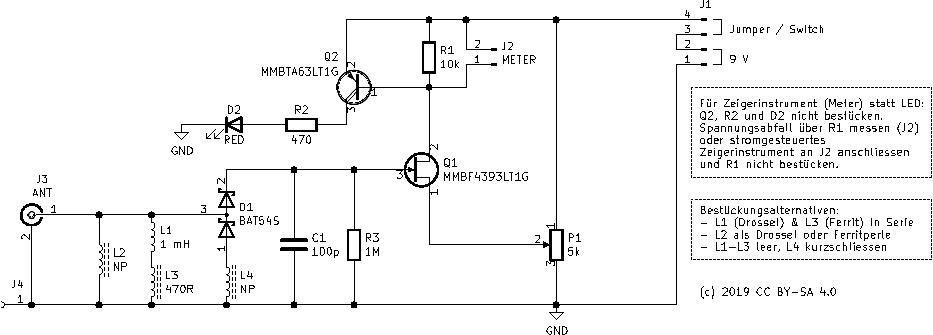
\includegraphics[width=\textwidth]{schaltung.pdf}
\caption{Schaltschema des HF-Spürers}
\label{fig:schematic}
\end{figure}

\section{Aufbau}
Der Aufbau erfolgt gemäss Abbildung \ref{fig:schematic}. Als Antenne dient ein
Draht von 30 -- 100~cm Länge, welcher an J3 gelötet wird (Beschriftung ``ANT''
auf Platinenrückseite; Pin im Zentrum verwenden, es kann zum Experimentieren
auch eine SMA-Buchse eingelötet werden).
% FIXME: Abbildung
Ein ebensolanges Gegengewicht ist notwendig, welches mit der Masse
verbunden wird (Loch mit Massensymbol verwendet). Die Schaltung benötigt eine Spannung von
9~V und wird über Pins 1 und 2 von J1, z.B. von einer 9~V Blockbatterie
gespiesen. Pins 3 und 4 dienen dem Ein- und Ausschalten; an sie kann ein Schalter
angeschlossen werden, oder aber die beiden Pins werden mit einem Jumper einfach
kurzgeschlossen. Die 3~mm LED kann, je nach Einsatz, auf der Vorder- oder der
Rückseite eingesetzt werden.  Abbildung \ref{fig:aufbau} zeigt eine fertig
bestückte Platine.

\begin{figure}[H]
    \begin{center}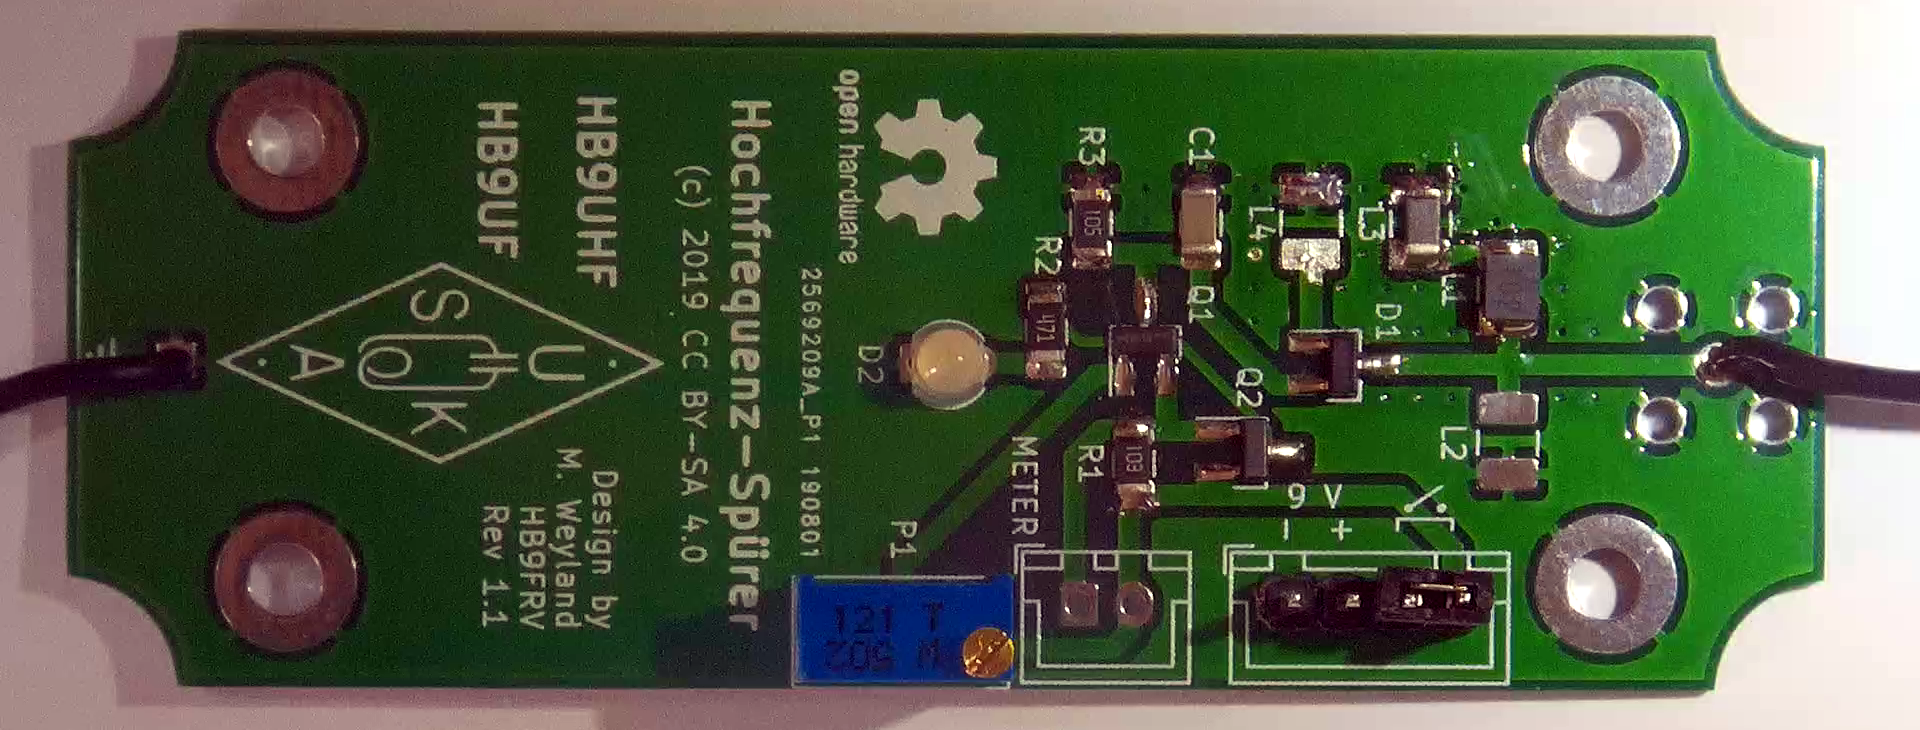
\includegraphics[width=0.6\textwidth]{foto.png}\end{center}
\caption{Fertig bestückte Platine.}
\label{fig:aufbau}
\end{figure}

Beim Einsatz eines
Netzteiles ist zu berücksichtigen, dass das Spiesekabel ebenfalls als Antenne
wirkt. Ausserdem darf ein solches Netzteil selbst keine Hochfrequenz produzieren,
da der HF-Spürer diese unweigerlich anzeigen würde. In Abwesenheit von
hochfrequenten Feldern wird schliesslich P1 aus der Nullstellung heraus (10 
Umdrehungen im Gegenuhrzeigersinn) im Uhrzeigersinn soweit erhöht, biss die LED
ganz schwach zu leuchten beginnt. Die Schaltung bezieht im Leerlauf ca. 2~mA.

\section{Stückliste}

\begin{center}\begin{tabular}{lllll}\toprule
    \textbf{Referenz} & \textbf{Bauteilwert} & \textbf{Gehäuse} & \textbf{Beschriftung} & \textbf{Bemerkung}\\\midrule
R1 & 10~k$\Omega$ & SMD 1206 & 103 & \\
R2 & 470~$\Omega$ & SMD 1206 & 471 & \\
R3 & 1~M$\Omega$  & SMD 1206 & 105 & \\
C1 & 100~pF       & SMD 1206 & (hellgrau) & \\
Q1 & MMBF4393LT1G & SMD SOT-23 & M6G & N Kanal J-FET\\ % FIXME check marking
Q2 & MMBTA63LT1G  & SMD SOT-23 & 2U & PNP Darlington\\ 
D1 & BAT54S       & SMD SOT-23 & WV4 & Schottky Diode\\ %  FIXME check marking
D2 & LED          & 3~mm bedrahtet & -- & Rot oder blau\\
L1 & 1~mH         & SMD 1210   & (breit) & \\
L3 & Ferritperle  & SMD 1206   & (schwarz) & \\
P1 & 5~k$\Omega$  & bedrahtet  & -- & 10 Umdrehungen\\\bottomrule
\end{tabular}\end{center}

Die Platine ist zur Monage in ein RND 455-00848 Metallgehäuse ausgelegt. Dazu
werden in den Deckel 4 Löcher für M3 Senkschrauben gebohrt, sowie ein 3~mm
Loch für die LED und zwei 1~mm Löcher für die beiden Antennendrähte. Der
Ein/Aus-Schalter und allenfalls ein 9~V DC Anschluss und das Potentiometer
können dann herausgeführt werden. Für eine steckbare Ausführung kann J1
mit einer JST XH Buchse bestückt werden.

\section{Justierung}
Vor der ersten Inbetriebnahme wird P1 ganz zurückgedreht (Gegen-Uhrzeigersinn).
Das Potentiometer hat keinen Anschlag, aber ein ganz leises Klicken beim
Drehen verrät, dass das Ende erreicht ist. Anschliessend wird die Schaltung gespiesen
bzw. eingeschaltet und sollte bei ausgeschalteter LED ca. 2~mA beziehen. P1
wird zur Justierung langsam in Abwesenheit von HF- und Störsignalen im
Uhrzeigersinn gedreht, bis die LED ganz leicht zu leuchten beginnt. Dieser
Arbeitspunkt ist Abhängig von der Eingangsspannung, d.h. beim Entladen der
Batterie ist allenfalls eine periodische Korrektur notwendig.

\newpage

\section{FIXME Rückseite}

Ideen:

\begin{itemize}
    \item Fotos, z.B. von der Deluxe Version oder Makroshots der einzelnen Bauteile
    \item Anwendung, z.B. NFC, HF CW, Handfunkgeräte, Störquellen
    \item Verbesserungsvorschläge, z.B. Spannungsregler, bessere Diode, Drossel.
    \item Mehr Infos zur Deluxe-Version (Bohrschablone, Anschluss-Schema usw.)
\end{itemize}
\end{document}



